\documentclass{beamer}
\usepackage{graphicx}
\usepackage{hyperref}
\usepackage{listings}
\usepackage{amsmath}

\title{KloudMinds: An AI-driven Cloud-Native File Management Service}
\author{KloudCrew}
\date{\today}

\begin{document}

\frame{\titlepage}

\begin{frame}
\frametitle{Introduction}
\begin{itemize}
    \item KloudMinds is an AI-driven cloud-native file management service.
    \item Leverages Kubernetes architecture to offer unparalleled flexibility, scalability, and security.
    \item Ensures automatic horizontal scaling, high availability, and reliability.
    \item Provides deep security and compliance measures that are typically absent in conventional cloud storage services.
\end{itemize}
\end{frame}

\begin{frame}
\frametitle{Core Features}
\begin{itemize}
    \item \textbf{Secure Storage}: Utilize robust security measures with Kubernetes secrets and config maps to ensure your data is safe.
    \item \textbf{Scalable Architecture}: Automatically scale your storage needs with Kubernetes' horizontal pod autoscaler.
    \item \textbf{Persistent Storage}: Reliable and persistent storage using Kubernetes Persistent Volumes (PVs) and Persistent Volume Claims (PVCs).
    \item \textbf{High Availability}: Ensure data availability and reliability with managed object storage (S3/MinIO) and metadata databases (MySQL).
\end{itemize}
\end{frame}

\begin{frame}
\frametitle{Innovative Features}
\begin{itemize}
    \item \textbf{AI-Powered Document Management}:
    \begin{itemize}
        \item \textbf{RAG Q\&A Retrieval}: Integrate with large language model APIs to enable intelligent retrieval-augmented generation (RAG) for advanced question-answering capabilities.
        \item \textbf{Document Summarization}: Automatically generate summaries of stored documents using state-of-the-art language models, saving time and improving productivity.
        % \item \textbf{Version Control}: Implement Git-like version management for documents, allowing users to track changes, revert to previous versions, and collaborate efficiently.
    \end{itemize}
\end{itemize}
\end{frame}

\begin{frame}
\frametitle{Comparison with Existing Solutions}
\begin{itemize}
    \item \textbf{Microsoft New Bing}: Focuses on web-based search and generation but lacks precision in retrieving proprietary knowledge.
    \item \textbf{OpenAI's ChatGPT \& GitHub Copilot}: Operate with limited data and knowledge scope.
    \item \textbf{Google Drive \& OneDrive}: Offer basic versioning and security features but fall short in performance, security, and functionality compared to KloudMinds.
\end{itemize}
\end{frame}

% \begin{frame}
% \frametitle{Advanced Capabilities}
% \begin{itemize}
%     \item \textbf{Real-Time Caching}: Improve performance with Redis-based caching for frequently accessed data.
%     \item \textbf{Monitoring and Logging}: Comprehensive monitoring and logging with Prometheus and Grafana for real-time insights and detailed analysis.
%     \item \textbf{Authentication and Authorization}: Secure access to your storage with dedicated authentication services and role-based access control.
% \end{itemize}
% \end{frame}

% \begin{frame}
% \frametitle{User Experience}
% \begin{itemize}
%     \item \textbf{Intuitive Interface}: User-friendly interfaces for web, mobile, and desktop platforms ensure a seamless and consistent user experience.
%     \item \textbf{Document Collaboration}: Enhance collaboration with features like shared access, version history, and real-time editing (planned for future releases).
%     \item \textbf{Customizable Settings}: Personalize your storage experience with flexible configuration options.
% \end{itemize}
% \end{frame}

% \begin{frame}
% \frametitle{Security and Compliance}
% \begin{itemize}
%     \item \textbf{Data Encryption}: Ensure data security with encryption at rest and in transit.
%     \item \textbf{Compliance}: Adhere to industry standards and regulations for data storage and management.
% \end{itemize}
% \end{frame}

% \begin{frame}
% \frametitle{Backup and Recovery}
% \begin{itemize}
%     \item \textbf{Data Backup}: Automated backup services to protect your data and ensure quick recovery in case of data loss (planned for future releases).
% \end{itemize}
% \end{frame}

\begin{frame}
\frametitle{Future Work}

\begin{figure}
    \centering
    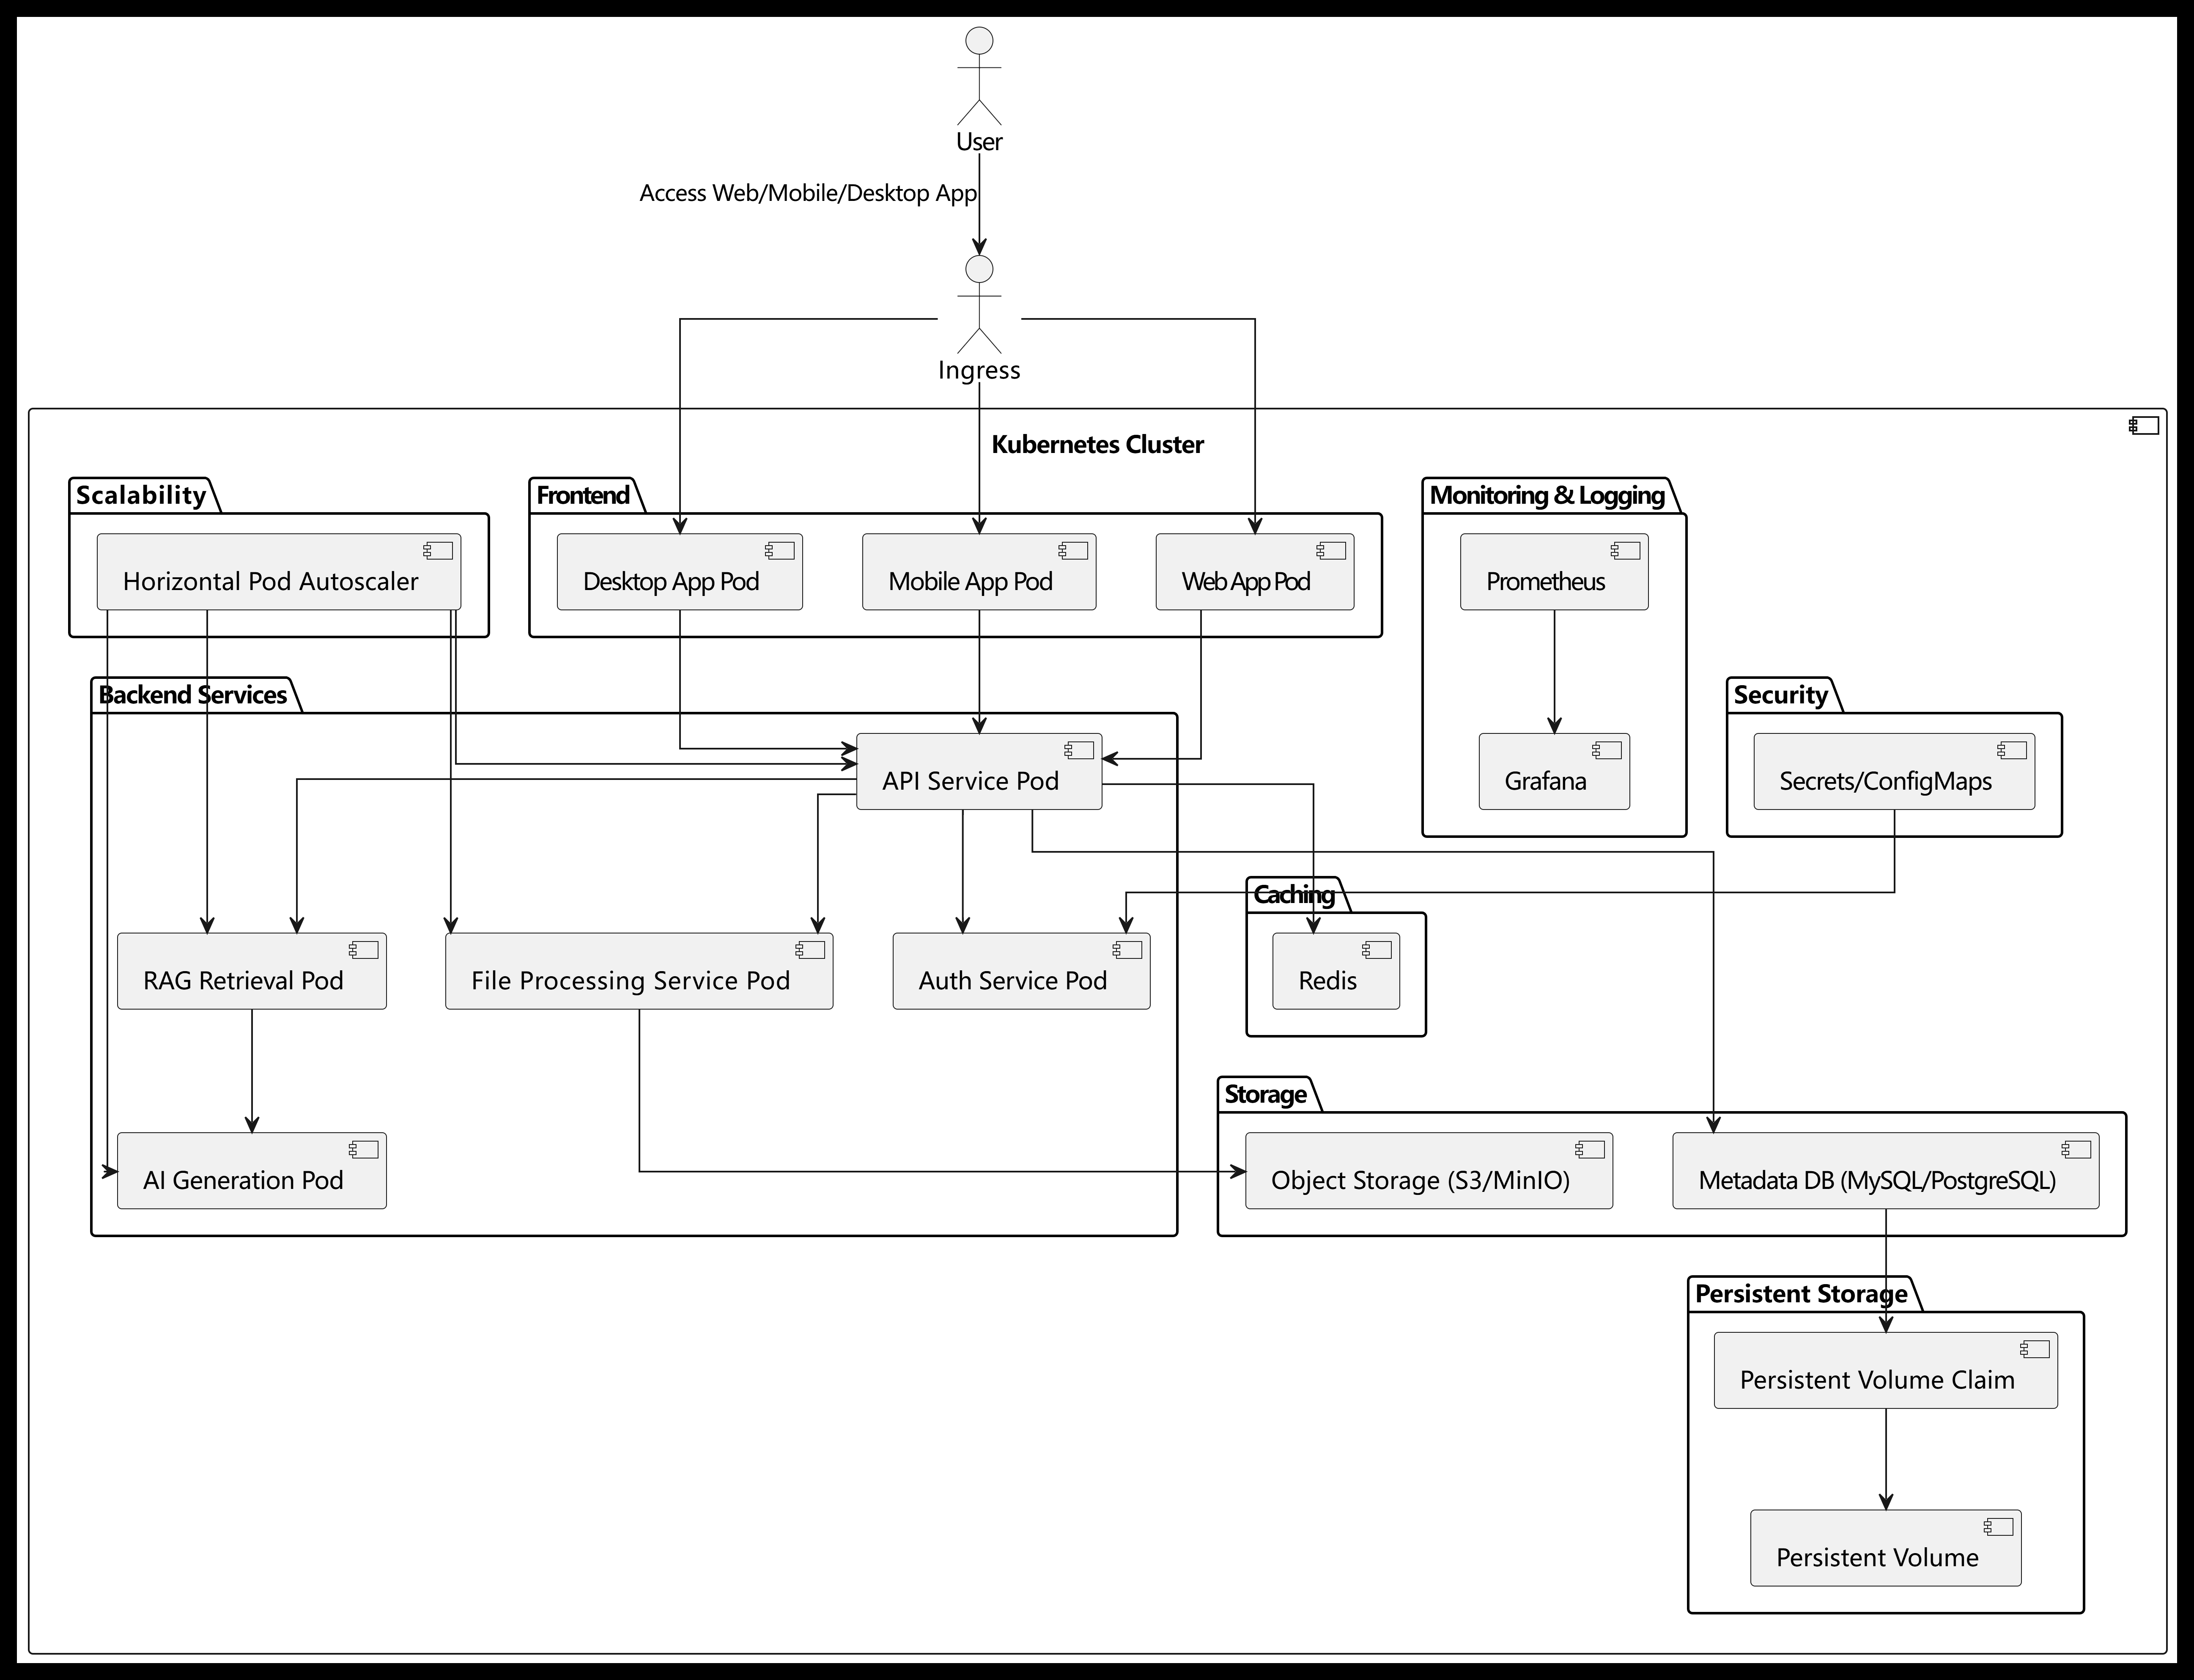
\includegraphics[width=0.9\linewidth]{1720778700094.jpg}
    \caption{Expected Architecture}
    \label{fig:my_label}
\end{figure}

\end{frame}

\begin{frame}
\frametitle{Future Work}
\begin{itemize}
    \item \textbf{Big Data}: Optimize computation speed, increase storage capacity, and enhance data security.
    \item \textbf{Large Language Models}: Improve the accuracy of responses in specialized domains by leveraging proprietary knowledge bases.
    \item \textbf{Applications}: Increase flexibility and ease of deployment for diverse applications.
    \item \textbf{Development}: Simplify component modifications, iterative development, and system expansion.
\end{itemize}
\end{frame}

\end{document}
